\xiti
\begin{xiaotis}

\begin{enhancedline}
\xiaoti{在 $\pxsbx ABCD$ 中:}
\begin{xiaoxiaotis}

    \xxt{已知周长为 28 cm, $AB = \exdfrac{3}{4} BC$, 求各边的长;}

    \xxt{已知 $\angle A + \angle C = 200^\circ$, 求各角的度数。}

\end{xiaoxiaotis}
\end{enhancedline}


\xiaoti{已知:$\pxsbx ABCD$ 和 $\pxsbx AEFD$ 如图。
    求证:$\triangle ABE \quandeng \triangle DCF$。
}

\begin{figure}[htbp]
    \centering
    \begin{minipage}[b]{7cm}
        \centering
        \begin{tikzpicture}
    \tkzDefPoints{0/0/B,  2.5/0/C, 0.3/1.5/A, 2.8/1.5/D, 0.8/1.0/E, 3.3/1.0/F}
    \tkzDrawPolygon(A,B,C,D)
    \tkzDrawPolygon(A,E,F,D)
    \tkzDrawPolygons(A,B,E  D,C,F)
    \tkzLabelPoints[left](A,B)
    \tkzLabelPoints[right](C,D)
    \tkzLabelPoints[below](E)
    \tkzLabelPoints[right](F)
\end{tikzpicture}


        \caption*{(第 2 题)}
    \end{minipage}
    \qquad
    \begin{minipage}[b]{7cm}
        \centering
        \begin{tikzpicture}[scale=0.4]
    \pgfmathsetmacro{\be}{2}
    \pgfmathsetmacro{\df}{3}
    % 角 1 = 60 度, 角 C = 120 度, 角 B = 角 D = 60 度,角 BAE = 角 FAD = 30 度
    \pgfmathsetmacro{\ab}{2 * \be} % 30 度角所对边为斜边一半
    \pgfmathsetmacro{\ad}{2 * \df}

    \tkzDefPoints{0/0/B, \ad/0/C}
    \tkzDefPoint(60:\ab){A}
    \tkzDefShiftPoint[C](60:\ab){D}

    \tkzDefPointBy[projection= onto B--C](A)  \tkzGetPoint{E}
    \tkzDefPointBy[projection= onto C--D](A)  \tkzGetPoint{F}
    \tkzDrawPolygon(A,B,C,D)
    \tkzDrawSegments(A,E  A,F)
    \tkzMarkRightAngle[size=.5](A,E,B)
    \tkzMarkRightAngle[size=.5](A,F,D)
    \tkzMarkAngle[size=0.8](E,A,F)
    \tkzLabelAngle[pos=1.5](E,A,F){$1$}
    \tkzLabelPoints[left](A,B)
    \tkzLabelPoints[right](C,D)
    \tkzLabelPoints[below](E)
    \tkzLabelPoints[right](F)
\end{tikzpicture}


        \caption*{(第 6 题)}
    \end{minipage}
\end{figure}


\xiaoti{求证:平行四边形对角线的交点到一组对边的距离相等。}

\xiaoti{已知: $E$、$F$ 是 $\pxsbx ABCD$ 的对角线 $AC$ 上的两点, 并且 $AE = CF$。
    求证: $BE = DF$。
}

\xiaoti{求证: 平行四边形一条对角线的两个端点到另一条对角线的距离相等。}

\xiaoti{如图,$\pxsbx ABCD$ 中,$AE \perp BC$,$AF \perp CD$, 垂足分别是 $E$、$F$,
    $\angle 1 = 60^\circ$, $BE = 2 \;\limi$, $DF = 3 \;\limi$,
    求各内角的度数与各边的长。
}


\xiaoti{}%
\begin{xiaoxiaotis}%
    \xxt[\xxtsep]{画一条直线和一条已知直线平行,并且距离为 20 mm 。这样的直线可以画几条?}

    \xxt{求作一条直线和两条已知平行线平行且距离等。}

\end{xiaoxiaotis}


\xiaoti{求证: 一组对边平行,一组对角相等的四边形是平行四边形。}

\xiaoti{}%
\begin{xiaoxiaotis}%
    \xxt[\xxtsep]{已知, $A$、$C$ 是直线 $l$ 同旁的两点, $AB \perp l$, $CD \perp l$,
        垂足分别是 $B$、$D$,且 $AB = CD$。 求证: $AC \pingxing l$(图甲);
    }

    \xxt{如果一块木板两边是直线,把两把曲尺的一边紧靠木板边缘,再看木板另一边缘对曲尺另一边上刻度是否相等,
        就可以判断木板的两个边緣是否平行。为什么(图乙)?
    }

\end{xiaoxiaotis}


\begin{figure}[htbp]
    \centering
    \begin{minipage}[b]{9.5cm}
        \centering
        \begin{minipage}[b]{4.5cm}
            \centering
            \begin{tikzpicture}
    \tkzDefPoints{0/0/B, 2/0/D, 0/1.5/A, 2/1.5/C, 3/0/M}
    \tkzDrawLines[add=0.4 and 0.4](B,D  A,C)
    \tkzLabelSegment[pos=1.5,right](B,D){$l$}
    \tkzDrawSegments(A,B  C,D)
    \tkzMarkRightAngle(A,B,D)
    \tkzMarkRightAngle(C,D,M)
    \tkzLabelPoints[above](A,C)
    \tkzLabelPoints[below](B,D)
\end{tikzpicture}


            \caption*{甲}
        \end{minipage}
        \quad
        \begin{minipage}[b]{4.5cm}
            \centering
            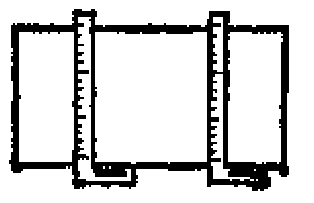
\includegraphics[width=4cm]{../pic/czjh1-ch4-xiti13-09-b}
            \caption*{乙}
        \end{minipage}
        \caption*{(第 9 题)}
    \end{minipage}
    \qquad
    \begin{minipage}[b]{4.5cm}
        \centering
        \begin{tikzpicture}
    \tkzDefPoints{0/0/A,  2.5/0/B, 3.3/1.5/C, 0.8/1.5/D}
    \tkzDefPointBy[projection= onto A--C](B)  \tkzGetPoint{M}
    \tkzDefPointBy[projection= onto A--C](D)  \tkzGetPoint{N}
    \tkzDrawPolygon(A,B,C,D)
    \tkzDrawSegments(A,C  B,M  B,N  D,M  D,N)
    \tkzMarkRightAngle[size=.2](B,M,A)
    \tkzMarkRightAngle[size=.2](D,N,C)
    \tkzLabelPoints[left](A,D)
    \tkzLabelPoints[right](B,C)
    \tkzLabelPoints[left=.3em](N)
    \tkzLabelPoints[right,yshift=-.3em](M)
\end{tikzpicture}


        \caption*{(第 11 题)}
    \end{minipage}
\end{figure}



\xiaoti{已知:$E$、$F$、$G$、$H$ 分别是 $\pxsbx ABCD$ 的边 $AB$、$BC$、$CD$、$DA$ 上的点,
    并且 $AE = CG$, $BF = DH$。 求证:四边形 $EFGH$ 是平行四边形。
}

\xiaoti{已知: $AC$ 是 $\pxsbx ABCD$ 的一条对角线,$BM \perp AC$, $DN \perp AC$,
    垂足分别是 $M$、$N$。 求证: 四边形 $BMDN$ 是平行四边形。
}

\xiaoti{已知:$\pxsbx ABCD$ 的对角线 $AC$ 上两点 $E$、$F$,且 $AE = CF$。
    求证: 四边形 $BFDE$ 是平行四边形。
}

\xiaoti{求证:平行四边形一组对角的平分线如果不在同一条直线上,那么它们互相平行。}


\xiaoti{求作 $\pxsbx ABCD$, 使}
\begin{xiaoxiaotis}

    \xxt{以已知点 $A$、$B$、$C$ 为顶点,这样的平行四边形可以作几个?写出其中一个的作法。}

    \xxt{$AB = a$, $BC = b$, $\angle ABC = \alpha$。}

\end{xiaoxiaotis}

\end{xiaotis}

